\documentclass[11pt]{article}
\usepackage{amssymb,amsmath}
\usepackage{mathrsfs}  
\usepackage{graphicx}
\usepackage[margin=2cm]{geometry}
\usepackage{tikz}
\usepackage[tikz]{mdframed}
\mdfdefinestyle{hlframe}{%      
frametitlebackgroundcolor   =black!15,%                                    
    backgroundcolor   =black!5,%                                               
    frametitlerule          =true,%                                            
    roundcorner     =10pt,%                                                
    middlelinewidth     =1pt,%                                             
    innermargin     =0.5cm,%                                               
    outermargin     =0.5cm,%                                               
    innerleftmargin     =0.5cm,%                                           
    innerrightmargin        =0.5cm,%                                       
    innertopmargin      =0.75\topskip,%                                    
    innerbottommargin   =0.75\topskip,%                                    
}
\usepackage{hyperref}
\hypersetup{
    colorlinks=true,
    linkcolor=blue,
    citecolor=red,
    filecolor=magenta,      
    urlcolor=blue
    }
\usepackage[nameinlink,capitalize]{cleveref}
\usepackage{algorithm}
\usepackage{algpseudocode}
\title{Hamiltonian solver}
\author{Eike Mueller, University of Bath}
\date{\today}
\begin{document}
\maketitle
We consider the following coupled system of time-dependent equations:
\begin{equation}
    \begin{aligned}
    \frac{\partial q}{\partial t} &= F_q(p,\xi;\theta_q) \\
    \frac{\partial p}{\partial t} &= F_p(p,\xi;\theta_p)
    \end{aligned}
\end{equation}
with initial conditions $q(0)=q_0$, $p(0)=p_0$. Here $q(t),p(t)\in\mathbb{R}^{n/2}$ are the dynamic variables, which are obtained by splitting the state $z(t)\in\mathbb{R}^n$ into two parts of equal size and $\xi\in \mathbb{R}^{n_{\text{ancil}}}$ are the ancillary variables. $\theta_q\in V_q$ and $\theta_p\in V_p$ are learnable parameters. The functions $F_q$ and $F_p$ could arise from a separable Hamiltonian
\begin{equation}
  H(q,p,\xi;\theta_q,\theta_p) = H_q(q,\xi;\theta_q) + H_p(p,\xi;\theta_p)
\end{equation}
i.e.
\begin{equation}
    \begin{aligned}
    F_q &= - \frac{\partial H}{\partial p} = - \frac{\partial H_p}{\partial p}\\
    F_p &=  \frac{\partial H}{\partial q} = \frac{\partial H_q}{\partial q}
    \end{aligned}
\end{equation}
A symplectic integrator is given by \cref{alg:symplectic_integrator}.
\begin{algorithm}
\caption{Symplectic integrator to compute $q(T), p(T)$ from $q_0,p_0$. \textbf{Input:} initial states $q_0,p_0$, final time $T$, number of timesteps $N_t$ \textbf{Output:} approximation $q_T,p_T\approx q(T), p(T)$ at final time $T$.}\label{alg:symplectic_integrator}
\begin{algorithmic}[1]
    \State{Set $\Delta t = T/N_t$}
    \State{Set $q^{(1/2)}=q_{0}+ \frac{\Delta t}{2} F_q(p_0,\xi;\theta_q)$, $p^{(0)} = p_0$}
    \For{$k=1,2,\dots,N_t$}
    \State{Set $p^{(k)} = p^{(k-1)}+\Delta t F_p(q^{(k-1/2)},\xi;\theta_p)$}    
    \If {$k<N_t$}
    \State{Set $q^{(k+1/2)} = q^{(k-1/2)}+\Delta t F_q(p^{(k)},\xi;\theta_q)$}
    \EndIf
    \EndFor
    \State{Set $q_T = q^{(N_t-1/2)}+\frac{\Delta t}{2} F_q(p^{(N_t)},\xi;\theta_q)$, $p_T=p^{(N_t)}$}
    \State {\Return $q_T, p_T$}
\end{algorithmic}
\end{algorithm}
For a given final time $T$ and number of timesteps $N_t$ the algorithm defines a mapping
\begin{equation}
    \begin{aligned}
\Phi: \mathbb{R}^{n/2}\times \mathbb{R}^{n/2} \times \mathbb{R}^{m} \times V_q \times V_p &\rightarrow \mathbb{R}^{n/2}\times \mathbb{R}^{n/2}\\
    q_0,p_0,\xi;\theta_q,\theta_p &\mapsto q_T, p_T
    \end{aligned}
\end{equation}
from the initial state $q_0,p_0$ to the (approximate) final state $q_T,p_T\approx q(T),p(T)$. This mapping is parameterised by the auxilliary state $\xi$ and the parameters $\theta_q,\theta_p$. We want to implement $\Phi$ in such a way that it is possible to back-propagate the output gradients $G_{q,T}=\frac{\partial J}{\partial q_T}$, $G_{p,T}=\frac{\partial J}{\partial p_T}$ to the gradients with respect to all inputs, i.e. $G_{q,0}=\frac{\partial J}{\partial q_0}$, $G_{p,0}=\frac{\partial J}{\partial p_0}$, $G_{\xi}=\frac{\partial J}{\partial \xi}$, $G_{\theta_q}=\frac{\partial J}{\partial \theta_q}$, $G_{\theta_p}=\frac{\partial J}{\partial \theta_p}$. The forward pass given by \cref{alg:symplectic_integrator_forward_pass}, which is essentially identical to \cref{alg:symplectic_integrator}.
\begin{algorithm}
\caption{Forward pass of function $\Phi(q_0,p_0,\xi;\theta_q,\theta_p)$. \textbf{Input:} initial states $q_0,p_0$, final time $T$, number of timesteps $N_t$ \textbf{Output:} approximation to $q(T), p(T)$ at final time $T$.}\label{alg:symplectic_integrator_forward_pass}
\begin{algorithmic}[1]
    \State{Set $\Delta t = T/N_t$}
    \State{Initialise $q\gets q_{0}+ \frac{\Delta t}{2} F_q(p_0,\xi;\theta_q)$, $p \gets p_0$}
    \For{$k=1,2,\dots,N_t$}
    \State{Update $p \gets p +\Delta t F_p(q,\xi;\theta_p)$}   
    \If {$k=N_t$} \State{Set $\rho=\frac{1}{2}$} \Else \State{Set $\rho=1$} \EndIf
    \State{Update $q \gets q+\rho \Delta t F_q(p,\xi;\theta_q)$}
    \EndFor
    \State {\Return $q_T=q$, $p_T=p$}
\end{algorithmic}
\end{algorithm}
The algorithm is written down schematically in \cref{fig:symplectic_dataflow}.
\begin{figure}
\begin{center}
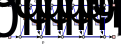
\includegraphics[width=0.75\linewidth]{symplectic_dataflow.pdf}
\caption{Flow of information in the symplectic integrator in \cref{alg:symplectic_integrator}}
\end{center}
\end{figure}

\begin{algorithm}
\caption{Backward pass of function $\Phi(q_0,p_0,\xi;\theta_q,\theta_p)$. \textbf{Input:} final states $q_T,p_T$ (as computed with \cref{alg:symplectic_integrator_forward_pass}) and corresponding gradients $G_{q,T}, G_{p,T}$, final time $T$, number of timesteps $N_t$. \textbf{Output:} gradients $G_{0,T}, G_{0,p}, G_{\xi}, G_{\theta_q}, G_{\theta_p}$.}\label{alg:symplectic_integrator_forward_pass}
\begin{algorithmic}[1]
    \State{Set $\Delta t = T/N_t$}
    \State{Initialise $q\gets q_{T}$, $p \gets p_T$}    
    \State{Initialise $G_q\gets G_{q,T}$, $G_p \gets G_{p,T}$}    
    \State{Initialise $G_\xi\gets 0$, $G_{\theta_q}\gets 0$, $G_{\theta_p}\gets 0$}
    \For{$k=N_t,N_t-1,\dots,2,1$}
    \If {$k=N_t$} \State{Set $\rho=\frac{1}{2}$} \Else \State{Set $\rho=1$} \EndIf
    \State{Update $q \gets q-\rho \Delta t F_q(p,\xi;\theta_q)$}
    \For {all variables $v\in \{p,\xi,\theta_q,\theta_p\}$}
        \State{Update $G_v\gets G_v + \rho \Delta t \frac{\partial F_q}{\partial v}(p,\xi;\theta_q,\theta_p)$}
    \EndFor    
    \State{Update $p \gets p -\Delta t F_p(q,\xi;\theta_p)$}
    \For {all variables $v\in \{q,\xi,\theta_q,\theta_p\}$}
        \State{Update $G_v\gets G_v + \Delta t \frac{\partial F_p}{\partial v}(q,\xi;\theta_q,\theta_p)$}
    \EndFor    
    \EndFor
    \State{Update $q \gets q-\frac{\Delta t}{2} F_q(p,\xi;\theta_q)$}
    \For {all variables $v\in \{p,\xi,\theta_q,\theta_p\}$}
        \State{Update $G_v\gets G_v + \frac{\Delta t}{2} \frac{\partial F_q}{\partial v}(p,\xi;\theta_q,\theta_p)$}
    \EndFor      
    \State {Set $G_{q,0}\gets G_q$, $G_{p,0}\gets G_p$}
    \State {\Return gradients $G_{q,0}$, $G_{p,0}$, $G_\xi$, $G_{\theta_q}$, $G_{\theta_p}$}
\end{algorithmic}
\end{algorithm}

\end{document}